\begin{figure}[t]
    \centering
    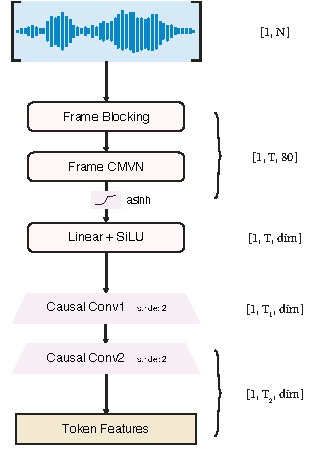
\includegraphics[width=.85\columnwidth]{figures/preprocessor-architecture.pdf}
    \caption{Audio preprocessor overview with tensor shapes, single-example. Dimensions $T = \lfloor \frac{N}{80} \rfloor$, $T_1 = \lceil \frac{T}{2} \rceil$, and $T_2 = \lceil \frac{T_1}{2} \rceil$}
    \label{fig:audio-preprocessor}
\end{figure}

\section{Approach}
\label{sec:approach}
Moonshine v2 consists of four high-level stages: an audio preprocessor, a
streaming encoder, an adapter, and a decoder. We start by detailing the audio
preprocessor.

\subsection{Audio preprocessor}
Our audio preprocessor is intentionally lightweight: it converts raw audio to a
50~Hz feature sequence (matching Whisper's feature rate) using simple operations
with no right context. Many of the frontend choices were informed guesses and
engineering intuition rather than a comprehensive ablation study; a full sweep
over alternative frontends is cost-prohibitive for us and out of scope for this
paper.

The original Moonshine model~\citep{jeffries2024moonshinespeechrecognitionlive}
used a full-attention encoder and a different frontend with an effective feature
rate of 41.6~Hz. In Moonshine v2 we standardize on 50~Hz features to align with
Whisper~\citep{radford2022robustspeechrecognitionlargescale} and to simplify
comparisons.

Specifically, the frontend processes audio by segmenting it into non-overlapping
80-sample windows (equivalent to 5~ms at 16~kHz), performing per-frame cepstral
mean and variance normalization (CMVN)~\citep{acero1995augmentedcepstralnorm},
and applying an $\operatorname{asinh}$ nonlinearity. The $\operatorname{asinh}$
function, like $\tanh$, is smooth and nearly linear around zero, but it
increases logarithmically for large values rather than saturating, which we
found balances compression and dynamic range effectively. Finally, two causal
stride-2 convolutions reduce the frame rate by approximately a factor of four,
yielding about 50 feature frames per second.

\subsection{Encoder}
The encoder is a standard Transformer stack with sliding-window self-attention.
Each layer attends to a fixed number of past frames (left context) and,
optionally, a small number of future frames (right context). We denote the
attention window as $(w_\text{left}, w_\text{right})$ in frames.

\paragraph{No positional embeddings (ergodic encoder).}
We do not use any absolute or relative positional embeddings in the encoder. As
a result, encoder computations are translation-invariant in time: for any local
window, the same function is applied regardless of where that window occurs in
the utterance. Informally, the encoder is \emph{ergodic} in the sense that it
has no explicit notion of absolute position; it can only infer structure from
the content of the local context provided by sliding-window attention.

In Moonshine v2, we use $(16,4)$ for the first two and last two encoder layers,
and $(16,0)$ for all intermediate layers. Since each encoder input frame
corresponds to 20~ms of audio (50~Hz), a right window of $w_\text{right}=4$
implies an algorithmic lookahead of $4\times20\,\mathrm{ms}=80\,\mathrm{ms}$: to
produce the representation at time step $t$ for layers with lookahead, the model
may use information up to frame $t+4$, i.e., up to 80~ms of future audio.

Layers with $(16,0)$ are strictly causal: their output at time $t$ depends only
on frames $\leq t$ (plus whatever future information has already been mixed into
the current frame by earlier lookahead layers). Overall, this design keeps
encoder lookahead bounded and small while still allowing limited future context
near the bottom and top of the stack.

\paragraph{Provisional vs. finalized encoder states.}
We note that the right-context layers also imply that, in steady state, a
\emph{finalized} representation for time step $t$ cannot be produced until
additional future audio has arrived. In our setting, a conservative bound is 16
frames of extra audio, i.e., $16\times20\,\mathrm{ms}=320\,\mathrm{ms}$ of
future context.

For applications such as live caption display, we can still decode from
\emph{provisional} (not-yet-finalized) encoder states: the newest suffix may be
less accurate, but as more audio arrives the provisional states are overwritten
by finalized ones and the displayed transcription naturally improves.

\subsection{Adapter}
The adapter bridges the ergodic encoder and the decoder. It adds a learned
positional embedding to the encoder outputs, and (when needed) applies a linear
projection so that the representation dimension matches the decoder dimension.
In other words, the encoder remains position-free, while the decoder receives
position-aware inputs.

\subsection{Decoder}
The decoder is a standard causal Transformer with rotary positional embeddings
(RoPE) in each layer~\citep{su2023roformerenhancedtransformerrotary}. It
autoregressively generates text tokens and cross-attends to the adapter
features.

While our ergodic streaming encoder makes the first usable features available
quickly (and thus TTFT can be very low), the decoder remains autoregressive:
generating a long transcript still requires a token-by-token loop, which adds
latency to the full output.

A fully ergodic, infinite-streaming alternative would be to predict directly
from encoder features using a linear classifier trained with
CTC~\citep{graves2006ctc}, or to use a monotonic transducer objective such as
RNN-T~\citep{graves2012rnnt} or Token-and-Duration Transducer
(TDT)~\citep{xu2023tdt}. Parakeet-class models follow this general direction
(CTC/RNN-T/TDT-style training and decoding) and shift much of the modeling
capacity into a larger encoder~\citep{rekesh2023fastconformer}. Marrying these
objectives with our position-free (ergodic) encoder is a promising direction
that we leave to future work.
